\documentclass[12pt,a4paper]{report}
% importation des packages
\usepackage[utf8]{inputenc}
\usepackage[francais]{babel}
\usepackage{graphicx}
\graphicspath{ {./images/} }
\usepackage{subcaption}


%hauts et bas de pages
\usepackage{fancyhdr}
\usepackage{color}
\usepackage[Glenn]{fncychap}
\pagestyle{fancy}
\lhead{Projet de Science des données}
\rhead{Groupe SantEconomie} 
\lfoot{License MIASHS}
\rfoot{2022/2023} 
\cfoot{\textbf{Page \thepage}}
\renewcommand{\headrulewidth}{1pt}
\renewcommand{\footrulewidth}{1pt}

\begin{document}

%------------------------------------------------premiere page
\begin{titlepage}

%logo paul valéry et logo projet
\begin{center}
\begin{figure}[h]
    \centering
    \begin{subfigure}{0.3\textwidth}
        \centering
        \includegraphics[width=\linewidth]{/Users/axel/Documents/Rapport_Projet/images/Logo_de_l'université_Paul_Valéry_-_Montpellier_3.jpg}
    \end{subfigure}
    \hspace{3,5cm}
    \begin{subfigure}{0.4\textwidth}
        \centering
        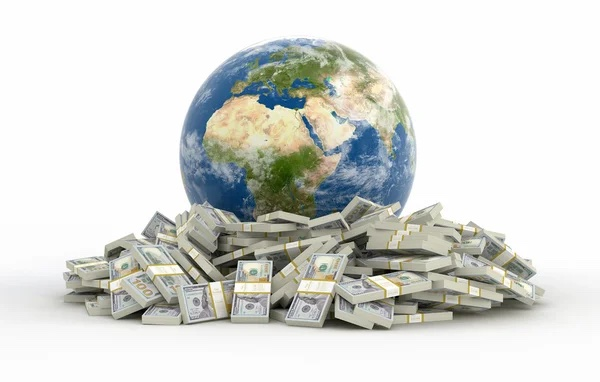
\includegraphics[width=\linewidth]{/Users/axel/Documents/Rapport_Projet/images/logo_projet.jpg}
    \end{subfigure}
    \label{fig:images}
\end{figure}

\medskip
{\Large{Universit\'{e} Paul Val\'{e}ry }}\\
\textsc{UFR 6}\\
 \vskip0.5cm
  \noindent {\textsc{\LARGE \textcolor{blue}{Licence MIASHS}}\\[1cm]}
\end{center}
\vskip0.5cm
\begin{center}
\textbf{Projet de science des donn\'{e}es}\\
\vskip0.5cm
%------------------------------------------------
\newcommand{\HRule}{\rule{\linewidth}{0.5mm}} 
	\HRule\\[0.2cm]
	{\huge\bfseries\textcolor{blue}{Projet SantEconomie\\[0.2cm]}}
	\HRule\\[1cm]
%------------------------------------------------
Par: \\
\small \bf{\ Girondin Audric, Can Arisoy Ivan, Duckes Jonathan, \\ Carot-Gelas Axel, Ravalisaona Malala, Abdallah Rachydah}
\end{center}
%------------------------------------------------
  \vspace{3mm}
  \centerline {\small \bf{\ Soutenue le $03/05/2022$}}
  \vspace{3mm}
  \centerline {\small \bf{\ Encadrants : $Sandra Bringay, Namrata Patel$}} 
%------------------------------------------------
\vskip2.5cm
\begin{center}
{\small{Année Universitaire : \textbf{2022-2023}}} \\
\end{center}

\end{titlepage}
%------------------------------------------------fin premiere page

% Insertion des tables de figures, de matieres et liste des tables
\newpage
    \tableofcontents % insertion de table des matières
    %\listoffigures % insertion de table des figures
    %\listoftables % insertion de liste des tableaux 


% Introduction Générale
\chapter{Introduction Générale}
\section{Contexte du projet}
	Ce module a pour objectif de nous apprendre à mener à bien un projet de groupe, de sa conception à sa livraison. La conception du projet s'est étalée sur deux semestres :
\begin{itemize}
    \item Le premier sera accès sur la rédaction d'un cahier des charges.
    \item Le second sur la réalisation du produit.
\end{itemize}

\section{Enjeux}
	Notre site a pour but de renseigner quiconque le souhaite, sur les données reliant la santé et l'économie de chaque pays. Pour cela, nous disposons de données concernant les facteurs suivants : 
\begin{itemize}
    \item Le PIB par habitant
    \item L'espérance de vie
    \item Les dépenses en santé
    \item Le taux d'obésité
\end{itemize}	

\section{Modèle de la base de donnée : MCD/MOD}

mettre les images
	
\section{Fonctionnalitées}
\subsection{Découvrez notre carte}
	Notre carte permet d'explorer le globe terrestre. L'utilisateur peut ensuite sélectionner un pays pour consulter le bilan des données dont nous disposons. 
\subsection{Comparez les pays}
	Le comparateur crée un graphique illustrant le facteur de deux pays choisis au préalable par l'utilisateur. Il est aussi possible de choisir le facteur parmi une liste. 
\subsection{Création d'un compte}
	L'utilisateur peut créer son compte sur notre site en choisissant son identifiant et son mot de passe. 
\subsection{Publiez votre article}
	Le site comporte la fonctionnalité de publier des articles en lien avec les données mises à disposition après validation de l'administrateur. Cette fonctionnalité n'est réservée qu'aux utilisateurs ayant un compte sur notre site.

\chapter{Travail réalisé}
retracer les push sur git 
problèmes rencontrés
bouts de code avec explications 
\section{Semaine 1}
\section{Semaine 2}
\section{Semaine 3}
\section{Semaine 4}
\section{Semaine 5}
\section{Semaine 6}
\section{Semaine 7}

% Ici on va inserer une figures
%\begin{figure}
%    \centering
%    \includegraphics[width=15cm, height=8cm]{image.png}
%    \caption{Titre de notre figures}
%    \label{fig:fig1}
%\end{figure}

% Ici on va inserer une tableau
%\begin{table}[h!]
%\caption{Titre du tableu}
%    \centering
%    \begin{tabular}{ |p{3cm}||p{3cm}|p{3cm}|p{3cm}|  }
% \hline
% \multicolumn{4}{|c|}{Country List} \\
% \hline
% Country Name or Area Name& ISO ALPHA 2 Code &ISO ALPHA 3 Code&ISO numeric Code\\
% \hline
% Afghanistan   & AF    &AFG&   004\\
% Aland Islands&   AX  & ALA   &248\\
% Albania &AL & ALB&  008\\
% Algeria    &DZ & DZA&  012\\
% American Samoa&   AS  & ASM&016\\
% Andorra& AD  & AND   &020\\
% Angola& AO  & AGO&024\\
% \hline
%\end{tabular}
%\end{table}

\chapter{Conclusion}
quelles ont été les difficultés,
quelles ont été nos facilités,
qu'est ce qu'on a appris, 
qu'est ce qu'on aurait aimé mieux faire ou pas eu le temps ect... \\
Lien de la vidéo youtube pour la soutenance

% Maintenant on va ajouter Bibliographie et réferences
%\begin{thebibliography}{}
%\bibitem{bib1}
%X. Liu, D. Yang, et A. E. Gamal, \textit{"Deep Neural Network Architectures for Modulation Classification"}. Preprint, submitted January 5, 2018.
%
%\bibitem{bib2}
%S. R. Tembo Mouafo, \textit{“Applications de l’intelligence artificielle à la détection et l’isolation de pannes multiples dans un réseau de télécommunications”}. IMT Atlantique sous le sceau de l'Université Bretagne Loire, Thèse soutenue le 23 janvier 2017.
%\end{thebibliography}

\end{document}
